% !TEX TS-program = XeLaTeX
% !TEX spellcheck = en-US
\documentclass[aspectratio=169]{beamer}

\usetheme{bi}

\title{Lecture 9:\\ Neural networks I}
\institute{GRA4160: Predictive modelling with machine learning}
\date{March 7th 2024}
\author{Vegard H\o ghaug Larsen}

\begin{document}

\maketitle

\frame{
	\frametitle{Plan for today:}
	\begin{itemize}
		\item Introduction to neural networks
		\item Single layer (feed forward) neural networks
		\item Fitting a Neural Network
		\item Backpropagation
		\item Stochastic gradient descent
	\end{itemize}
}

\frame{
	\frametitle{Introduction to neural networks}
	\begin{itemize}
		\item A neural network is a computational system that is inspired by the structure and function of the human brain
		      \pause
		\item It consists of many interconnected processing units, called neurons, that work together to solve complex problems
		      \pause
		\item Each neuron receives input from other neurons, processes that input, and then produces an output that is sent to other neurons
		      \pause
		\item By combining and processing information in this way, a neural network can learn to recognize patterns and make predictions
	\end{itemize}
}

\frame{
	\frametitle{Single layer (feed forward) neural networks}

	\begin{itemize}
		\item A single layer neural network is a model that takes a set of $p$ input variables $X=(X_1,X_2,...,X_p)$
		      \pause
		\item The NN is a nonlinear function $f(X)$ that maps the input variables to an output variable $Y$
		      \pause
		\item The weights $w_1,w_2,...,w_p$ are the parameters of the model, controlling the strength of the relationship between the input variables and the output variable
		      \pause
		\item Given a nonlinear activation function $g(X)$, the model can be written as a sum of $K$ activation functions
	\end{itemize}
	\[ Y = f(X) = \beta_0 + \sum_{k=1}^K\beta_k g\left(w_{k0} + \sum_j^pw_{kj}X_j\right) \]
}

\frame{
\frametitle{Neural network with a single hidden layer}
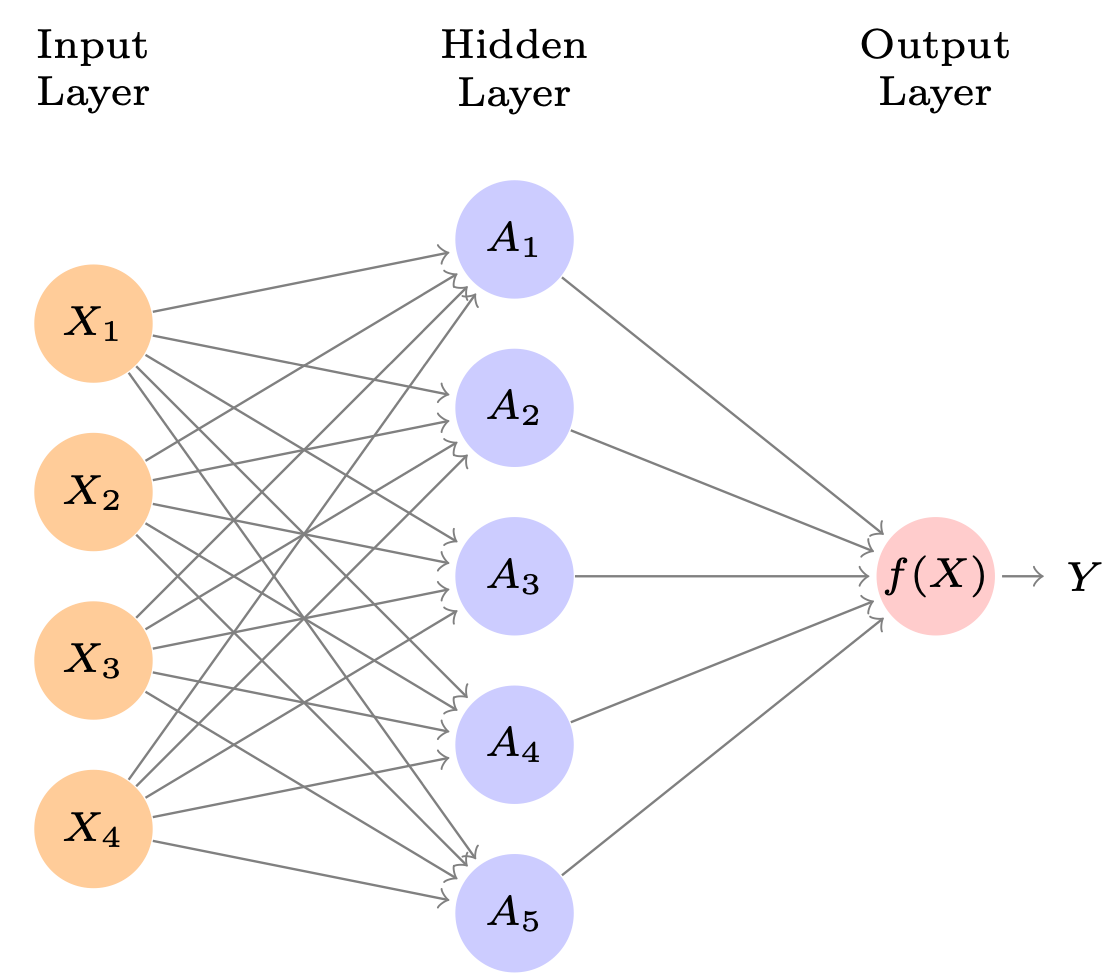
\includegraphics[scale=0.19]{figures/single_layer_NN.png}\\
{\footnotesize Source: An Introduction to Statistical Learning with Applications in R, James, Witten, Hastie and Tibshirani, 2013}
}

\frame{
	\frametitle{Hidden units and the output layer}
	The network is built up in two steps:
	\begin{enumerate}
		\item Specify the number of hidden units $K$ and the activation function $g(X)$ and we can calculate $K$ activations in the hidden layer as
		      \[A_k = h_k(X) = g\left(w_{k0} + \sum_j^pw_{kj}X_j\right) \]
		      \pause
		\item The $K$ activations feed into the output layer, which is a linear function of the activations
		      \[ f(X) = \beta_0 + \sum_{k=1}^K\beta_k A_k \]
	\end{enumerate}
}

\frame{
	\frametitle{What does the activation function look like?}
	Activation functions are used to introduce non-linearity and enable the network to learn complex patterns in the input data. Here are some common activation functions used in neural networks:
	\begin{enumerate}
		\item The sigmoid function (we also used this for logistic regression)
		      \[ g(z) = \frac{1}{1+e^{-z}} \]
		      \pause
		\item Rectified Linear Unit (ReLU)
		      \[ g(z) = \max(0, z) \]
		      \pause
		\item Softmax
		      \[ g(z_i) = \frac{\exp(z_i)}{\sum(\exp(z_j))} \]
	\end{enumerate}
}

\frame{
\frametitle{Sigmoid vs ReLU}
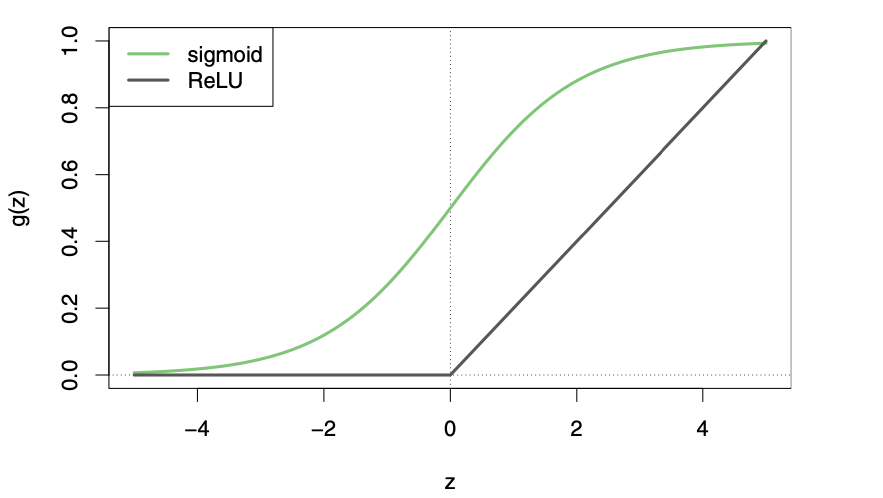
\includegraphics[scale=0.35]{figures/sigmoid_vs_relu.png}\\
{\footnotesize Source: An Introduction to Statistical Learning with Applications in R, James, Witten, Hastie and Tibshirani, 2013}
}

%\frame{
%	\frametitle{Multi-layer neural networks}
%	\begin{itemize}
%		\item A multi-layer neural network is a neural network with more than one hidden layer
%		\pause
%		\item Modern neural networks typically have more than one hidden layer
%		\pause
%		\item The hidden layers are used to learn more complex patterns in the data
%		\pause
%		\item The number of hidden layers and the number of hidden units in each layer are hyperparameters that can be tuned
%	\end{itemize}
%}

%\frame{
%	\frametitle{NN with two hidden layers and multiple outputs}
%	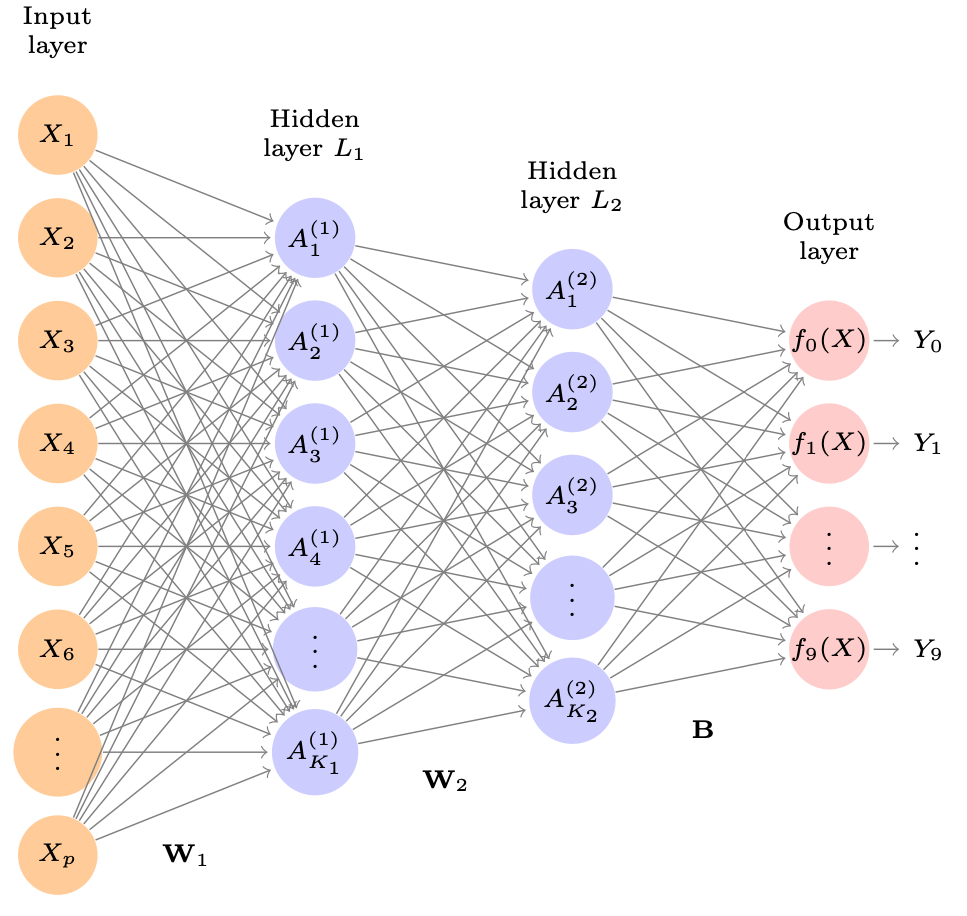
\includegraphics[scale=0.19]{figures/multilayer_NN.png}\\
%	{\footnotesize Source: An Introduction to Statistical Learning with Applications in R, James, Witten, Hastie and Tibshirani, 2013}
%}

%\frame{
%	\frametitle{The perceptron}
%	\begin{itemize}
%		\item ...
%	\end{itemize}
%}

%\frame{
%	\frametitle{The multilayer perceptron}
%	\begin{itemize}
%		\item ...
%	\end{itemize}
%}

\frame{
	\frametitle{Fitting a Neural Network}
	We can fit the parameters of a neural network by minimizing a cost function (nonlinear least squares)

	\[ \min_{w_k,\beta} \frac{1}{2}\sum_{i=1}^n \left( y_i - f(x_i) \right)^2 \]

	where

	\[ f(X) = \beta_0 + \sum_{k=1}^K\beta_k g\left(w_{k0} + \sum_j^p w_{kj}X_j\right) \]

	\pause

	This is a nonlinear optimization problem, and it is not straightforward to solve.
}

\frame{
	\frametitle{Gradient descent}
	We can use gradient descent to find the optimal parameters. Let´s put all the parameters in one vector $\theta$ and define the cost function as

	\[ L(\theta) = \frac{1}{2}\sum_{i=1}^n \left( y_i - f_\theta(x_i) \right)^2 \]

	\pause
	Then, to find the optimal parameters, we can use gradient descent to minimize the cost function $L(\theta)$ by the following iterative update rule:
	\begin{enumerate}
		\item Let $\theta^t$ be a vector of all the parameters in the system at iteration $t$. Start with an initial guess $\theta^0$
		      \pause
		\item Update the parameters according to the following rule: $\theta^{t+1} = \theta^t + \delta$, where $\delta$ is a vector that reflects a small change in the parameters such that
		      \[ L(\theta^{t+1})<L(\theta^{t}) \]
		\item Repeat until convergence
	\end{enumerate}
}

\frame{
\frametitle{How do we know how to update the parameters (what is $\delta$)?}

We need to calculate the gradient of the cost function $L(\theta)$ with respect to the parameters $\theta$:

\[ \nabla L(\theta^m) = \left.\frac{\partial L(\theta)}{\partial \theta}\right|_{\theta=\theta^m} = \left.\frac{\partial}{\partial \theta} \frac{1}{2}\sum_{i=1}^n \left( y_i - f_\theta(x_i) \right)^2\right|_{\theta=\theta^m} \]

\pause
$\nabla L(\theta^m)$ gives us the directions to move $\theta$ so as to decrease the objective $L(\theta)$\\
\pause
\smallskip
Given a learning rate $\eta$, we can use the gradient to update the parameters as follows:
\[ \theta^{t+1} = \theta^t - \eta \nabla L(\theta^t) \]
\pause
The gradient packs all the partial derivatives into a single vector: $\nabla L = \left[ \frac{\partial L}{\partial \beta_k}, \frac{\partial L}{\partial w_{kj}} \right]^T$
}

\frame{
	\frametitle{Backpropagation}
	The cost function $L(\theta)$ is a sum of squared errors, $L(\theta) = \sum_i^n L_i(\theta)$ where $L_i(\theta) = \frac{1}{2}\left( y_i - f_{\theta}(x_i) \right)^2$.\\
	\pause
	\smallskip
	The expression $\nabla L(\theta^m)$ can be calculated using the chain rule. The partial derivatives of the cost function with respect to the parameters are given by
	\pause
	\[ \frac{\partial L_i(\theta)}{\partial \beta_k} = \frac{\partial L_i(\theta)}{\partial f_\theta(x_i)} \cdot \frac{\partial f_\theta(x_i)}{\partial \beta_k} = - (y_i - f_\theta(x_i))\cdot g(z_{ik})\]
	\[ \frac{\partial Li(\theta)}{\partial w_{kj}} = \frac{\partial L_i(\theta)}{\partial f_\theta(x_i)} \cdot \frac{\partial f_\theta(x_i)}{\partial g(z_{ik})} \cdot \frac{\partial g(z_{ik})}{\partial z_{ik}} \cdot \frac{\partial z_{ik}}{\partial w_{kj}}  = - (y_i - f_\theta(x_i))\cdot\beta_k\cdot g'(z_{ik})x_{ij} \]
	\pause
	We assigns a fraction of the residual, $(y_i - f_\theta(x_i))$, to each of the parameters via the chain rule. This is called backpropagation.
}

\frame{
	\frametitle{Stochastic gradient descent (SGD)}
	\begin{itemize}
		\item SGD is a method for minimizing a cost function by iteratively moving in the direction of steepest descent as defined by the negative of the gradient
		      \pause
		\item In contrast to batch gradient descent, which computes the gradient of the cost function over the entire dataset, SGD computes the gradient on a single training example at a time
		      \pause
		\item This makes SGD much faster than batch gradient descent, but it also means that SGD is much noisier
		      \pause
		\item The noise can be reduced by averaging the gradients over several training examples
	\end{itemize}
}

\end{document}